\subsection{System design}

\paragraph{} The system is broken up into several components of increasing specificity (i.e. Participant $\in$ Pool $\in$ Blockchain $\in$ Global). Each component exists in a set under it's parent. The system can be described in the following terms and relationships:

\paragraph{Global} 

\begin{itemize}
  \item $\mathbb{H}$ - Global \textbf{h}ash rate
  \item $S_B$ - \textbf{S}et of \textbf{b}lockchains
  \item $T$ - \textbf{t}ime
\end{itemize}

\paragraph{Blockchain}

\begin{itemize}
  \item $\mathbb{R}$ - Block \textbf{r}eward
  \item $b$ - \textbf{B}lock time
  \item $S_P$ - \textbf{S}et of \textbf{p}ools
\end{itemize}

\paragraph{Pool}

\begin{itemize}
  \item $C$ - total \textbf{c}hunks
  \item $c$ - Available \textbf{c}hunks
  \item $H$ - \textbf{H}ash rate
  \item $t$ - \textbf{T}rade intervals 
  \item $r$ - Tax \textbf{r}ate
  \item $p_{p}$ - \textbf{P}ool sell \textbf{p}rice
  \item $R$ - \textbf{R}eward per chunk 
    \begin{equation} \label{equation:chunkreward}
      R = \frac{\mathbb{R}}{c} \times \frac{H}{\mathbb{H}}
    \end{equation}
  \item $P_p$ - \textbf{S}et of \textbf{p}articipants
\end{itemize}

\paragraph{Participant}

\begin{itemize}
  \item $x$ - Owned chunks
  \item $p_s$ - \textbf{S}ale \textbf{p}rice
  \item $y$ - Wanted chunks
  \item $p_p$ - \textbf{B}uying \textbf{p}rice
\end{itemize}

\begin{equation} \label{equation:tax}
  amountTaxable(x) = x \times p_s \times r
\end{equation}

\begin{align} \label{equation:profitpurchase}
  \begin{split}
    profit_{purchase} = &\; (x + y) \times R \\
    &\; - amountTaxable(x) \\
    &\; - amountTaxable(y) \\
    &\; - y \times p_b
  \end{split}
\end{align}

\begin{align} \label{equation:profitheld}
  \begin{split}
    profit_{held} = &\; x \times R \\
    &\; - amountTaxable(x)
  \end{split}
\end{align}

\begin{equation} \label{equation:profitsale}
  profit_{sale} = (y \times p_s)
\end{equation}

\paragraph{} At time $I_0$, all participants begin with $x = 0$ and a randomized amount of funds and the pool begins will $c = C$. Between each interval $I_i$ to $I_{i + t}$, participants will have an opportunity to initiate an auction for any of the available chunks $c$ from the pool at a starting rate of $p_p$ or from any of the other participants at their set price $p_s$ while keeping in mind their potential profit from Equations \ref{equation:profitpurchase} and \ref{equation:profitheld}. Finally, a tax is deducted from each participant according to Equation \ref{equation:tax} where $x = participant.x$ at $I_{i + t}$.

\subsection{Simulation}

\paragraph{} A basic functional implementation of the simulation has been completed, available at \url{https://github.com/hans-m-song/harbergers-tax}. The simulation is an implementation of the pseudocode below, with Algorithm \ref{algorithm:trade} being called at intervals based on the pool parameters. In order to simulate the rewards, Algorithm \ref{algorithm:reward} emulates the reward and distribution at each block time if the pool was successful in mining a new block.

\begin{algorithm}[H]
  \caption{Reward system for pool participants, executed at blockchain defined intervals}
  \label{algorithm:reward}
  \begin{algorithmic}[1]
    \Procedure{reward}{$P, p, r$} \Comment{$P \gets$ participants, $p \gets$ pool parameters, $r \gets$ reward}
      \State{$leftover \gets r$}
      \For{$participant \in P$}
        \State{$amount \gets p.\textsc{shareCalc}(participant.ownedChunks)$} \Comment{Share based on pool policy}
        \State{$participant.funds \gets participant.funds + amount$}
        \State{$leftover \gets leftover - amount$}
      \EndFor
      \State{$p.funds \gets p.funds + leftover$}
    \EndProcedure
  \end{algorithmic}
\end{algorithm}

\begin{algorithm}[H]
  \caption{Executed at pool defined intervals}
  \label{algorithm:trade}
  \begin{algorithmic}[1]
    \Procedure{trade}{$P, p$}  \Comment{$P \gets$ participants, $p \gets$ pool}
      \For{$seller \in P$}
        \State{$\textsc{auction}(seller, seller.price, P, \textsc{null})$}
      \EndFor
      \For{$taxee \in P$} \Comment{Taxation}
        \While{$taxee.funds < (taxee.ownedChunks \times taxee.price \times p.taxRate)$}
          \State{$taxee.ownedChunks \gets taxee.ownedChunks - 1$}
          \State{$p.availableChunks \gets p.availableChunks + 1$}
        \EndWhile
        \State{$amount \gets taxee.ownedChunks \times taxee.price \times p.taxRate$}
        \State{$taxee.funds \gets taxee.funds - amount$}
        \State{$p.funds \gets p.funds + amount$}
      \EndFor
    \EndProcedure
    \Procedure{auction}{$P$, $s$, $p$, $b$} \Comment{$P \gets$ bidders, $s \gets$ seller, $p \gets$ current price, $b \gets$ last bidder}
      \If{$P = \emptyset$}
        \State{$\textsc{transact}(s, b, p)$}
        \State{\Return}
      \EndIf
      \State{$maxBidder \gets b$}
      \State{$maxBid \gets p$}
      \For{$bidder \in P$}
        \State{$bid \gets bidder.\textsc{bid}(p)$}
        \If{$bid > maxBid$}
          \State{$maxBid \gets bid$}
          \State{$maxBidder \gets bidder$}
        \EndIf
      \EndFor
      \State{$P' \gets \emptyset$}
      \For{$bidder \in P$}
        \If{$bidder.$\textsc{canParticipate}$(seller.price)$}
          \State{$B \gets B \cup bidder$}
        \EndIf
      \EndFor
      \State{\Return $\textsc{auction}(P', s, maxBid, maxBidder)$}
    \EndProcedure
    \Procedure{transact}{$b, s, p$} \Comment{$b \gets$ buyer, $s \gets$ seller, $p \gets$ price}
      \State{$b.funds \gets b.funds - p$}
      \State{$b.ownedChunks \gets b.ownedChunks + 1$}
      \State{$s.funds \gets s.funds + p$}
      \State{$s.ownedChunks \gets s.ownedChunks - 1$}
    \EndProcedure
  \end{algorithmic}
\end{algorithm}

\subsection{Results}

\subsubsection{Data Collection}

\paragraph{Parameters} The following parameters were used to run the simulation for a single pool:

\begin{itemize}
  \item The computational power of each chunk was equal
  \item Block reward $\mathbb{R} = 10$
  \item Block time $b = 1s$
  \item Trade interval $t = 0.2s$
  \item Total chunks $C = 100$
  \item Tax rate $r = 0.02$
  \item Pool's share of global hash rate $\frac{H}{\mathbb{H}} = 0.3$
  \item Number of participants $P_p.length = 100$
\end{itemize}
The simulation ran for 100 rounds (i.e. 100 chances for the pool to earn the reward), in which the reward was received 31 times. Each participant started with a random amount of funds and 0 owned chunks while the pool started with all 100.

\paragraph{Collection} Each change to every participants balance was recorded along with timestamp, the number of blocks moved, and a reason. Additionally, general metrics on performance such as time take, number of transactions that occurred were recorded.

\paragraph{Postprocessing} Since all events happen asynchronously, transactions and reward distribution can occur anytime within the trade interval. Hence, the occurrence of block purchases and occurrence of rewards was binned based on trade interval and block interval respectively.

\subsubsection{Analysis}

\paragraph{} It can be seen from Figure \ref{figure:balances} below that the general trend of all participants is positive with significant jumps when a reward is earned. This indicates the tax rate or reward could be adjusted or more time is required to bring the system closer to equilibrium.

\begin{figure}[H]
  \centering
  \caption{Balances of all participants, excluding pool}
  \label{figure:balances}
  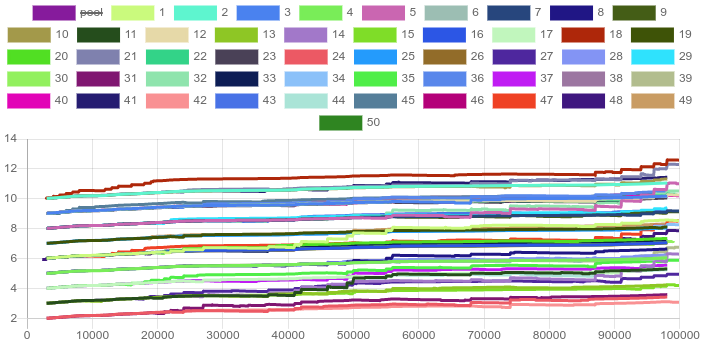
\includegraphics[width=\linewidth]{media/fig-balances}
\end{figure}

\paragraph{} From Figure \ref{figure:balances-pool} It can be seen that the pool's profits greatly outpace the growth of participants. This is primarily due to the pool possessing a large portion of the chunks which indicates the pricing of chunks or the decision making process for participants needs to be adjusted.

\begin{figure}[H]
  \centering
  \caption{Balances of all participants, pool inclusive}
  \label{figure:balances-pool}
  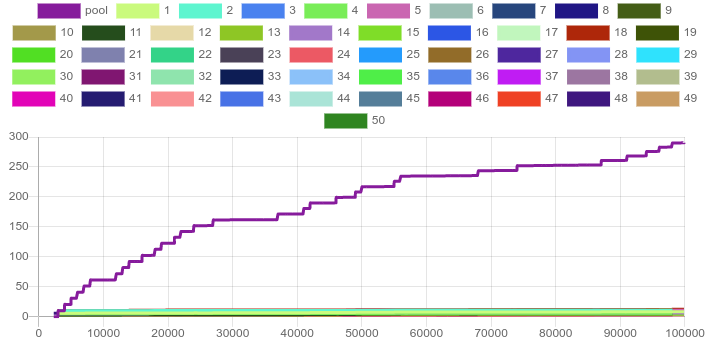
\includegraphics[width=\linewidth]{media/fig-balances-pool}
\end{figure}

\paragraph{} The occurrence of rewards can be seen in Figure \ref{figure:rewards}. The rewards occur as expected, with 31 rewards from the 100 total chances.

\begin{figure}[H]
  \centering
  \caption{Rewards earned by pool during game}
  \label{figure:rewards}
  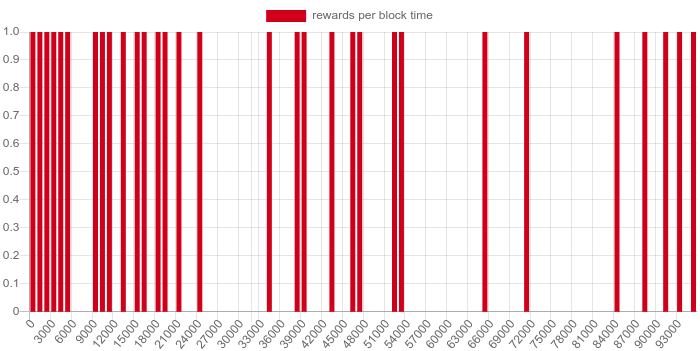
\includegraphics[width=\linewidth]{media/fig-rewards}
\end{figure}

\paragraph{} The frequency of block purchases per trade interval can be seen in Figure \ref{figure:blocks} with a high of 4 blocks in a single interval. While frequency of purchases slightly increases later on, the low amount of purchases may indicate the pricing needs to be adjusted.

\begin{figure}[H]
  \centering
  \caption{Blocks transferred throughout game}
  \label{figure:blocks}
  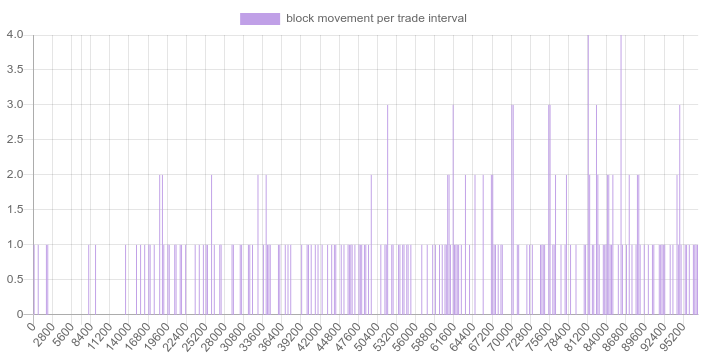
\includegraphics[width=\linewidth]{media/fig-blocks}
\end{figure}